\documentclass[linenumbers,twocolumn]{aastex631}
% \documentclass[linenumbers]{aastex631}

% Packages
\usepackage[utf8]{inputenc}
\usepackage{graphicx}
\usepackage{amsmath}
\usepackage{amssymb}
\usepackage{enumitem}
\usepackage{ulem}
\usepackage{hyperref}

% Editing commands
\newcommand{\mm}[1]{{\textcolor{purple}{\bf #1}}}

% Make upright subscripts and superscripts in Mathmode.
\def\subinrm#1{\sb{\mathrm{#1}}}
{\catcode`\_=13 \global\let_=\subinrm}
\mathcode`_="8000
\def\supinrm#1{\sp{\mathrm{#1}}}
{\catcode`\^=13 \global\let^=\supinrm}
\mathcode`^="8000
\def\upsubscripts{\catcode`\_=12 } \def\normalsubscripts{\catcode`\_=8 }
\def\upsupscripts{\catcode`\^=12 } \def\normalsupscripts{\catcode`\^=7 }

\newcommand{\vdag}{(v)^\dagger}
\newcommand\aastex{AAS\TeX}
\newcommand\latex{La\TeX}

% Title
\shorttitle{Deriving the Shock Crossing Time}
\shortauthors{Moss M.} 

\begin{document}

\upsubscripts
\upsupscripts

\title{Deriving the Shell Crossing Time as a Function of the Density}

\correspondingauthor{Michael Moss}
\email{mikejmoss3@gmail.com}

\begin{abstract}
The goal of this derivation to estimate the time it will take a reverse shock to cross incoming ejecta material.

\end{abstract}

\section{Introduction}
{
    In the refreshed shock model, the wind of a GRB can be separated into two regions, (i) early outflow launched with $\bar{\Gamma}\sim150$ and (ii) later ejecta launched launched with $\bar{\Gamma}\sim15$. The early material is responsible for producing the prompt emission and the afterglow continuum emission. The later ejecta will eventually catch up to the early ejecta as it sweeps up circumburst medium and decelerates. When the later ejecta catches up and collides with the early material, a ``refreshed'' shock occurs, injecting energy into the front of the outflow and may be witnessed as bumps in the afterglow light curves (potentially in the optical regime). In this work, we would like to estimate the time it takes the incoming energy injected from the later ejecta to be distributed across the newly shocked material. This timescale should be dominated by the shell crossing time $t_{\Delta }$, where we model the incoming late ejecta as a shell with width $\Delta$, density $n_4$, and Lorentz factor $\gamma_{4}\sim15$ (see Figure \ref{fig: schematic} for a schematic). 

    To estimate $t_{\Delta}$, we must estimate the density of the rapid material ($n_4$) and the material which the late ejecta is colliding with ($n_1$).
}

\section{Estimating Density of Zone 1 Material}
{
    The material that the late ejecta is colliding with is composed of early ejecta material that has been crossed by the reverse shock and has time had time to relax. The average particle density of this material $n_1$ (fluid frame) can be approximated as,

    \begin{align}
        n_{ej}(t) &= n_{1}(t) = \frac{E_{iso}\Gamma(t)}{4\pi m_p c^2 \Gamma_0 R(t)^2 \Delta_1(t)} \label{eq: dens estim} \\
    \end{align}

    where $R(t)$ is the distance of the material from the central engine, $E_{iso}$ is the isotropic equivalent energy, $\Gamma_0$ is the initial bulk Lorentz factor of the ejecta, and $\Gamma(t)$ is the bulk Lorentz factor as a function of time (all in the central engine frame). $\Delta_1(t)$ is the initial width of the material. 

    $\Delta_1(t)$ can take two extremes, if we assume that the early material relaxes as it propagates along the jet then $\Delta_1(t) \approx R(t)/\Gamma_1^2(t)$, and the density approximations becomes

    \begin{align}
        n_{1,min}(t) = \frac{E_{iso}\Gamma(t)}{4\pi m_p c^2 \Gamma_0 R(t)^3} \label{eq: dens estim min} \\
    \end{align}

    In the other extreme, if the material does not relax and the width of the material is approximately $\Delta \sim \beta_0 ct_{inj}$ where $t_{inj}$ is the duration of the injection time and $\beta_0 = \sqrt{1 - 1/\Gamma_0^2}$. This makes the approximation of the density 

    \begin{align}
        n_{1,max}(t) = \frac{E_{iso}\Gamma(t)}{4\pi m_p c^3 \Gamma_0 R(t)^2 t_{inj}} \label{eq: dens estim max} \\
    \end{align}

    We can estimate this density using a fiducial values $E_{iso} = 10^{53}$ erg/s, $\Gamma_0 = 150$, $R(t_{coll}) = 10^{17}$ cm, $\Gamma (t_{coll}) = 5$, and $t_{inj} = 20$ sec, which leads to a density estimate of $n_{1,min}=1.8\times10^{2}$ cm$^{-3}$ and $n_{1,max} = 3 \times 10^{7}$ cm$^{-3}$.
}

\section{Estimating the Shell Crossing Time}
{
    Following Sari and Piran 1995 (hereafter SP95), we can describe the width of the incoming late ejecta shell with respect to the density of the material, 

    \begin{align}
        \Delta &= \frac{E_{late,iso}}{4 \pi m_p c^2 \gamma_4^2 R^2 n_4} \label{eq: delta}
    \end{align}

    where $E_{iso,late}\sim10^{52}$ erg is the isotropic equivalent energy of the late material. Figure \ref{fig: shell width} shows $\Delta$ as a function of $n_4$. Following SP95, the time it takes an incoming relativistic shell to be crossed by a reverse shock is given by the expression, 

    \begin{align}
        t_{\Delta} = \frac{\Delta}{c(\beta_4 - \beta_2)} \left(1-\frac{\gamma_4 n_4}{\gamma_3 n_3}\right)
    \end{align} 

    where $\beta_i = \sqrt{1 - 1/\gamma_i^2}$.

    \begin{figure}[t!]
        \centering
        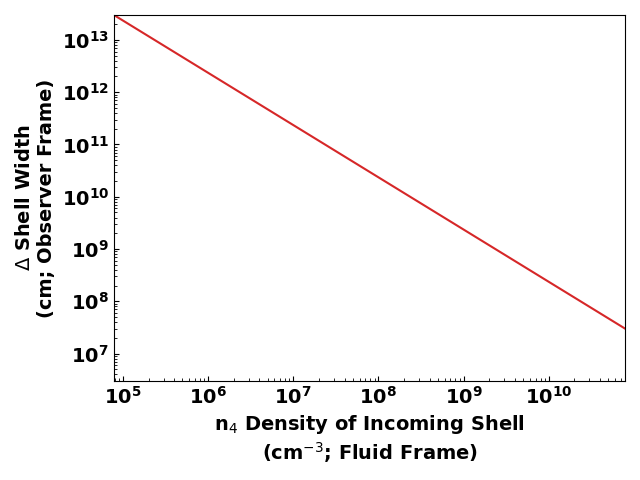
\includegraphics[width=0.45\textwidth]{shell-width.png}
        \caption{Late ejecta shell width $\Delta$ as a function of the density of the material (see Equation \ref{eq: delta}) }
        \label{fig: shell width}
    \end{figure}

    The shell crossing time depends on the density ratio $f = n_4/n_1$, where in this scenario $n_1 = n_{3,SP}$ found earlier. If $\gamma_4^2 \gg f$, the we are in a relativistic regime and the shell crossing time can be expressed as 

    \begin{align}
        t_{\Delta} = \Delta \gamma_4 \frac{\sqrt{f}}{2c}
    \end{align}

    Note, in this formalism, if $n_4> 2 n_1 / \gamma_4$, then the shock crosses the shell faster than the speed of light. 

    If $f\gg\gamma_4^2$, then the reverse shock is in a Newtonian regime and the shell crossing time is expressed as

    \begin{align}
        t_{\Delta} = \sqrt{\frac{9}{14}}\Delta\gamma_4\frac{\sqrt{f}}{c}
    \end{align}

    In Figure \ref{fig: shell cross time}, the shell crossing time $t_{\Delta}$ is shown as function of the shell width. There are two limits on the width of the late ejecta. The minimum width $\Delta_{4,min} = \beta c t_{inj}$, while the maximum width is determined by how much the late shell spreads out by the time it reaches the collision radius. We can estimate the spread by considering two particles, one launched with $\Gamma$ and the other launched with $\Gamma + \delta\Gamma$, we can then find the distance between the two particles $\delta R = \Delta_4$ at a radius $R$, which can be shown to be, 

    \begin{align}
        \Delta_4 = R \frac{\delta \Gamma}{\Gamma^3}
    \end{align}

    Looking at Figure \ref{fig: shell cross time}, the maximum $\Delta_{4,max}/c \sim 10^2$, which corresponds to a spread of Lorentz factors of 

    \begin{align}
        \delta \Gamma &\lesssim (\Delta_{4,max}/c) * (\Gamma^3 / R)\\
        &\approx 1 
    \end{align}

    For $\Gamma = 10$ and $R = 10^{17}$ cm.


    \begin{figure}[t!]
        \centering
        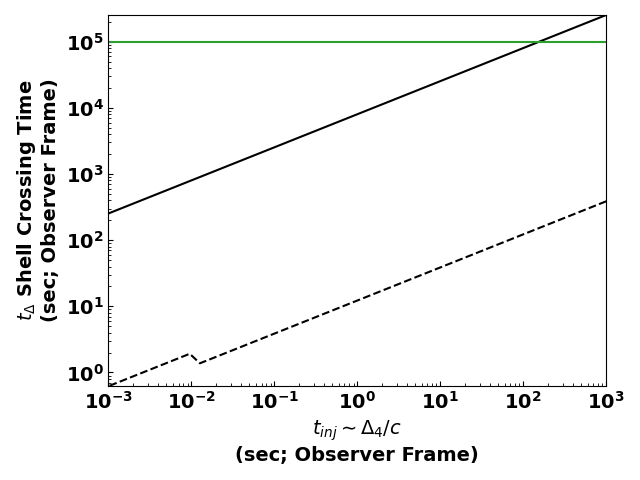
\includegraphics[width=0.45\textwidth]{shell-width-vs-cross-time.png}
        \caption{The shell crossing time as a function of the late ejecta shell width $\Delta$.}
        \label{fig: shell cross time}
    \end{figure}

    % \begin{figure}[t!]
    %     \centering
    %     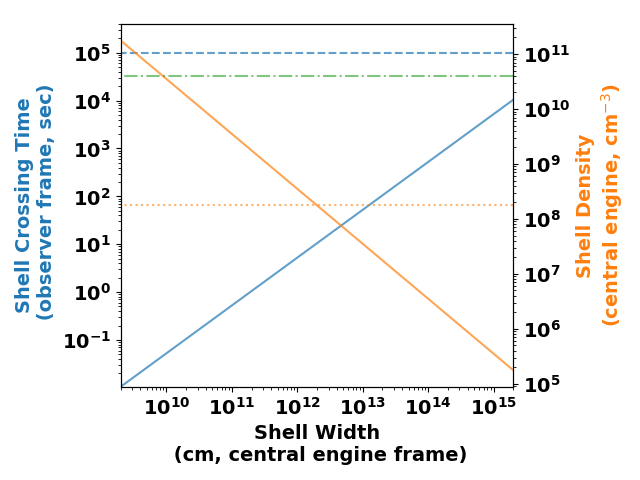
\includegraphics[width=0.45\textwidth]{shell-cross-time.png}
    %     \caption{Shell crossing time as a function of the density of the late ejecta material responsible for the refreshed shocks. The estimated density (which is likely an underestimate) is shown by the orange, dashed line and is estimated as $n_4 \sim 7.8 \times 10^{6}$ cm$^{-3}$. The green line indicates $10^{5}$ seconds, which is the approximate rise time of the bumps in optical afterglow of GRB030329.}
    %     \label{fig: shell cross time}
    % \end{figure}
}

    % \begin{figure*}[t!]
    %     \centering
    %     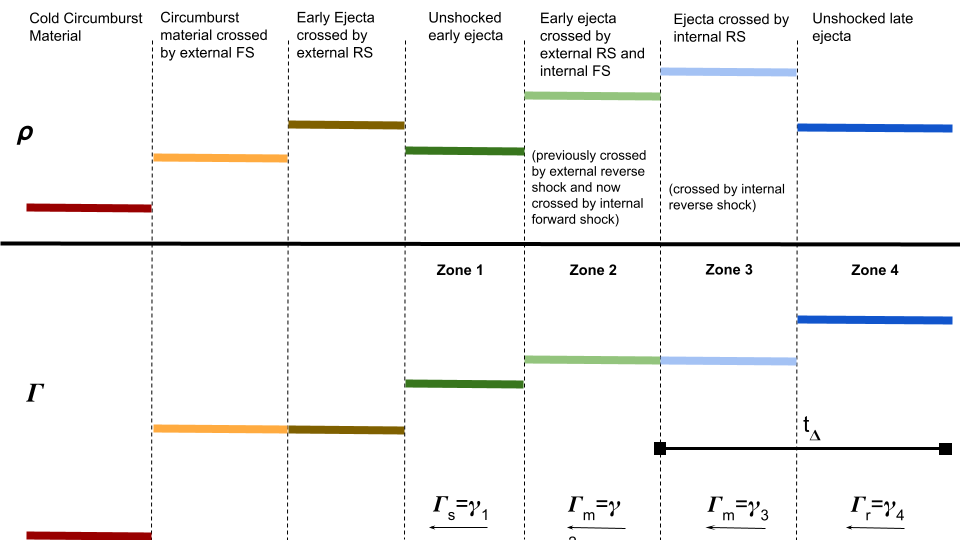
\includegraphics[width=0.7\textwidth]{schematic-pre-rs-complete.png}\\
    %     \vspace{1cm}
    %     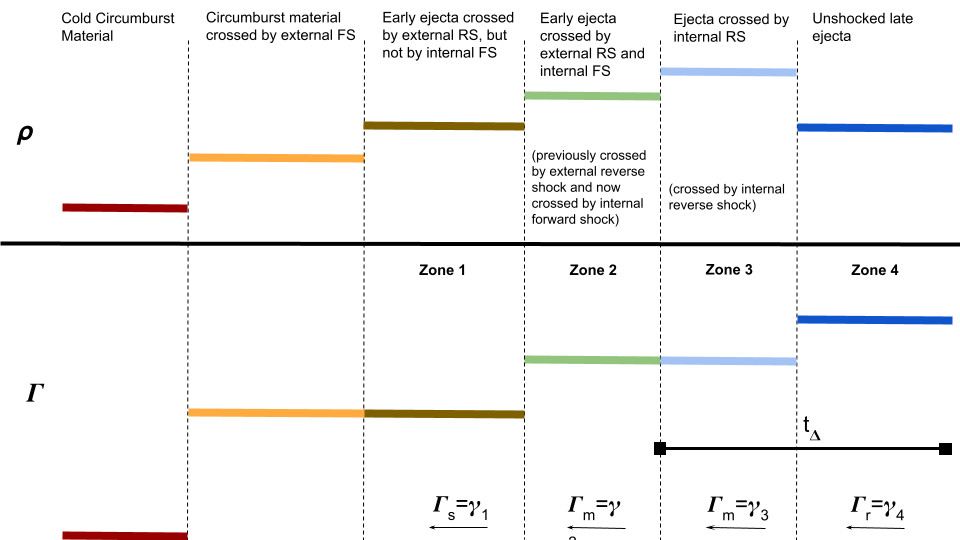
\includegraphics[width=0.7\textwidth]{schematic-aft-rs-complete.png}
    %     \caption{Schematic of the scenario (in the central engine frame). There are two ``reverse shocks'' in question, the reverse shock arising from the bulk of the jet decelerating as it sweeps up circumburst medium, which will be referred to as the external reverse shock, and an internal reverse shock arising from the deceleration of the incoming later ejecta decelerating as it rams the material in front of it (which happens to be the material previously crossed by the external reverse shock). The top panel shows a the situation we encounter if the late ejecta catches up to early material before the external reverse shock completely crosses the early material. It is more common that we will be in the case where the late material is colliding with early that has already been completely crossed by the external reverse shock (bottom panel).}
    %     \label{fig: schematic}
    % \end{figure*}

\end{document}
